\documentclass[12pt,a4paper]{article} 

\usepackage[utf8]{inputenc} % set input encoding (not needed with XeLaTeX)

%%% Examples of Article customizations
% These packages are optional, depending whether you want the features they provide.
% See the LaTeX Companion or other references for full information.


\usepackage{graphicx} % support the \includegraphics command and options
\graphicspath{ {./Figures/} }


%%% PACKAGES
\usepackage{booktabs} % for much better looking tables
\usepackage{array} % for better arrays (eg matrices) in maths
\usepackage{paralist} % very flexible & customisable lists (eg. enumerate/itemize, etc.)
\usepackage{verbatim} % adds environment for commenting out blocks of text & for better verbatim
\usepackage{subfig} % make it possible to include more than one captioned figure/table in a single float
% These packages are all incorporated in the memoir class to one degree or another...

%%% HEADERS & FOOTERS
\usepackage{fancyhdr} % This should be set AFTER setting up the page geometry
\pagestyle{fancy} % options: empty , plain , fancy
\renewcommand{\headrulewidth}{0pt} % customise the layout...
\lhead{}\chead{}\rhead{}
\lfoot{}\cfoot{\thepage}\rfoot{}



%%% ToC (table of contents) APPEARANCE
\usepackage[nottoc,notlof,notlot]{tocbibind} % Put the bibliography in the ToC
\usepackage[titles,subfigure]{tocloft} % Alter the style of the Table of Contents
\renewcommand{\cftsecfont}{\rmfamily\mdseries\upshape}
\renewcommand{\cftsecpagefont}{\rmfamily\mdseries\upshape} % No bold!

% ADDITIONAL PACKAGES	
\usepackage{float}
\usepackage{indentfirst} % indenting the first paragraph
\usepackage[left=2.54 cm, right=2.54 cm, top=2cm, bottom = 2 cm]{geometry} % Set page margins
\usepackage{mcite} % multiple citations
\usepackage{tocloft} % dots in table of contents
\renewcommand{\cftsecleader}{\cftdotfill{\cftdotsep}} % dots in table of contents
\usepackage{amsmath}
\usepackage{mathtools}
\usepackage[version=4]{mhchem}
\usepackage{array}
\usepackage{adjustbox}
\usepackage[utf8]{inputenc}
\usepackage{tikz}
\DeclareMathOperator{\sign}{sign}
\DeclareMathOperator{\argmax}{argmax}
\DeclareMathOperator{\argmin}{argmin}
\usepackage{tikz,pgfplots}
\pgfplotsset{compat=1.18} 
\usepackage{titlesec}
\usepackage{enumitem}
\titleformat{\section}
  {\normalfont\fontsize{12}{15}\bfseries}{\thesection}{1em}{}
\usepackage[noadjust]{cite}
%%% END Article customizations



\begin{document}


\begin{center}
\textbf{MTech Project Proposal}
\end{center}

\par\noindent\rule{\textwidth}{0.5pt}

\vspace{\baselineskip}
% title
\section{Title : \textnormal{Your Project Title Name}}

% project particulars
\section{Project Particulars}
\begin{enumerate} [label=(\Alph*)]
    \item \textbf{Project area and sub-areas:}  write area and subareas names here
   % \item \textbf{Duration (in months):} 11 
\end{enumerate} 


% student and mentor particulars
\section{Student and Mentor Particulars}
\begin{enumerate} [label=(\Alph*)]
    \item \textbf{Student Name:} your name
    \item \textbf{Student Roll Number:} your roll number
    \item \textbf{Immediate Supervisor:} supervisor full name
    \item \textbf{Mentor Name(s):} mentor full name(s)
\end{enumerate} 

% project summary
\section{Project Summary}
write your text here..

(approximately 200 words; Overall project motivation, problem, scope, goals, and deliverables)

% objectives
\section{Objectives} \label{sec:Obj}
 List here objectives (at least 3 objectives) to solve the problem
\begin{enumerate}
\item write text here
\item write text here
\end{enumerate}
% current state of the art
\section{Current State of The Art}


Please provide the current state of the art related to the proposed project. This involves describing the different methods, datasets and challenges associated with the proposed project in the literature. Please cite references in the appropriate paragraph or sentences. For example: \cite{Elgamal}.

% work plan
\section{Work Plan}
Work plan describes methods and approaches to achieve the stated objectives in Section \ref{sec:Obj}. Each objective will be divided into specific work packages. Each work package may include the following: Rationale for the work-package, data science/AI algorithms to be used, experiments to be performed and rationale behind the design of experiments, and metrics to be used to evaluate different experiments, etc. 

\section{Data Sets}
Please provide description of data sets to be used in this project. Do you have data sets with you or is the data in the public domain? If the data will be generated by you via a set of simulations, please provide details of how will you generate the data, choice of experimental conditions for the generation of the data, how will you ensure that the experiments emulate the real-world scenario. If you are using an industrial data set (which cannot be shared), the performance of different methods and/or proposed solution(s) in the thesis must be provided in relative terms along with appropriate masking. If you are using data from the public domain, provide the link. 

\section{Expected deliverables/outcomes}
Please provide 4-5 bullet points describing the expected outcome(s) of this project that can be quantitatively measured at the end of the project. 

\section{Significance of the expected outcome(s) with respect to the state-of-the-art in 
the field}
Discuss the impact of the expected project outcome(s) on the current state of knowledge in the field.


\section{Implementation arrangements proposed for the project (linkages and management structure) }

Provide a plan of action for implementing the project. For example, what is the plan to collect relevant data, gain requisite domain knowledge (if required), etc.


\section{Resource Requirements and their availability}
Software and hardware requirements and their availability should be listed here.


\section{Risks}
What are the risks involved in the project from the completion perspective ?



\section{Gantt chart}  

Provide a timeline and milestones for each work package using a Gantt Chart. An example is given in Figure \ref{fig:ganntex}.

\begin{figure}[h!]
    \centering
    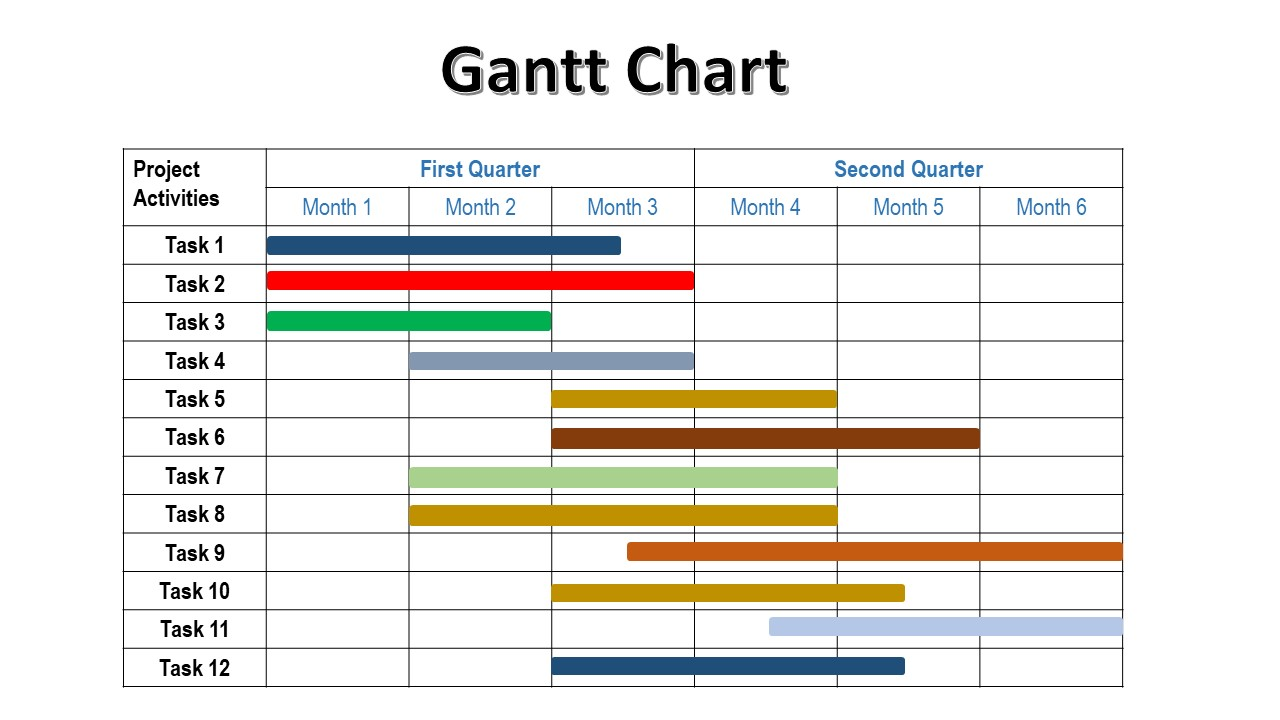
\includegraphics[width=0.85\textwidth]{Figures/GanntChart.jpg}
    \caption{Project Timeline}
    \label{fig:ganntex}
\end{figure}

\pagebreak

\bibliographystyle{IEEEtran}
\bibliography{reflist}


\newpage

\begin{center}
    \textbf{Appendices}
\end{center}

\section*{Appendix 1: Example of a Table }

\begin{table}[h]
\caption{Example of a Table in LaTeX}

\begin{center}
\begin{tabular}{ |c|c|c|c| } % 4 c = 4 columns
 \hline % Horizontal line
 \textbf{Heading 1} & \textbf{Heading 2} & \textbf{Heading 3} & \textbf{Heading 4}\\ 
 \hline % Horizontal line
 Item11 & Item12 & Item13 & Item24 \\ % \\ implies end of current row
 Item21 & Item22 & Item23 & Item24 \\ 
 \hline
\end{tabular}
\end{center}

\label{tab:ex}
\end{table}

\noindent Table \ref{tab:ex} is an example of a table in LaTeX. 

\section*{Appendix 2: Example of a Figure }

\begin{figure}[h!]
    \centering
    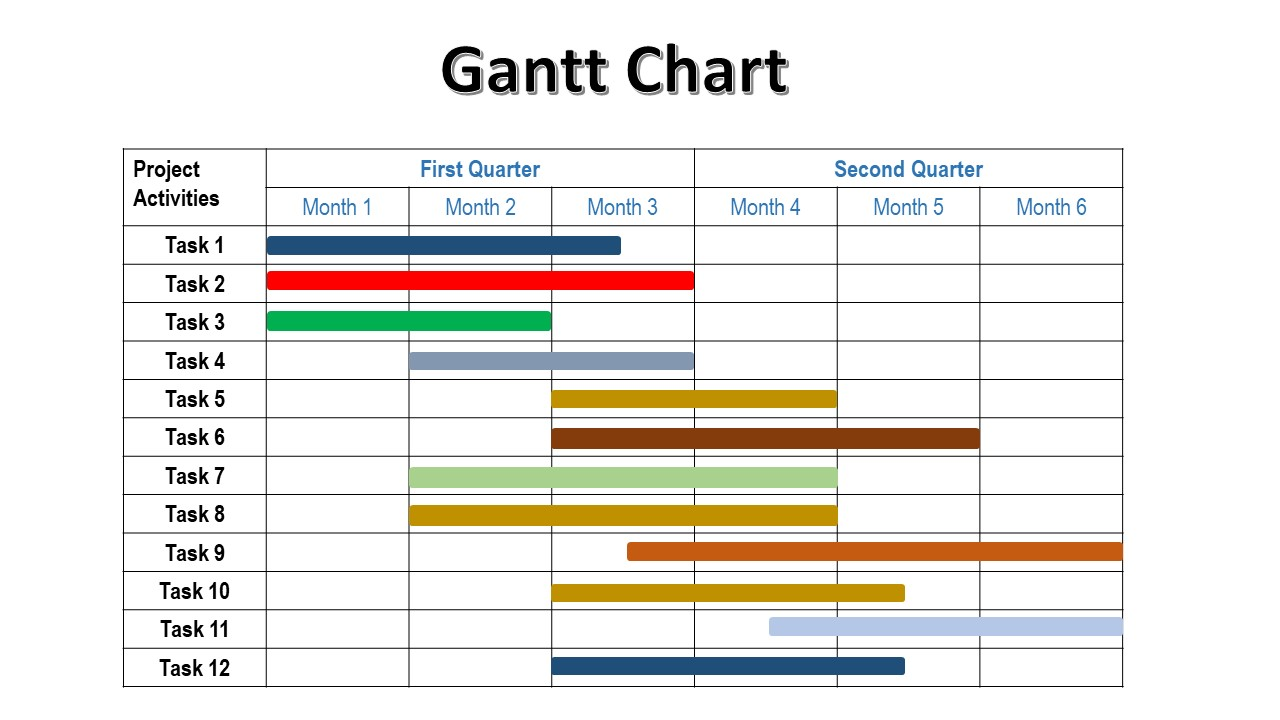
\includegraphics[width=0.85\textwidth]{Figures/GanntChart.jpg}
    \caption{Example of a Figure in LaTeX}
    \label{fig:gannt}
\end{figure}

Figure \ref{fig:gannt} is an example of a figure in LaTex.


\end{document}